\subsection{Kennlinien der Hochvakuumdiode} 
Aus den Tabellen (\ref{taba1} - \ref{taba5}) sind die darauf folgenden 
Abbildungen (\ref{pica1} - \ref{pica5}) erstellt worden.
\begin{table}[h!]
	\begin{center}
		\begin{tabular}{cc}
			Anodenspannung [V] & Anodenstrom [mA]\\ \hline
			10	&0,044\\
			20	&0,088\\
			30	&0,108\\
			40	&0,119\\
			50	&0,126\\
			60	&0,128\\
			70	&0,132\\
			80	&0,135\\
			90	&0,138\\
			100	&0,141\\
			110	&0,144\\
			120	&0,146\\
			130	&0,147\\
			140	&0,149\\
			150	&0,150\\
			160	&0,151\\
			170	&0,152\\
			180	&0,154\\
			190	&0,155\\
			200	&0,156\\
			210	&0,157
		\end{tabular}
		\caption{Kennlinie 1 (Heizwerte: 4,2V; 2,1A)}
		\label{taba1}
	\end{center}
\end{table} \begin{table}[h]
	\begin{center}
		\begin{tabular}{cc}
			Anodenspannung [V] & Anodenstrom [mA]\\ \hline
			10	&0,049\\
			20	&0,123\\
			30	&0,181\\
			40	&0,232\\
			50	&0,263\\
			60	&0,281\\
			70	&0,302\\
			80	&0,310\\
			90	&0,322\\
			100	&0,330\\
			110	&0,336\\
			120	&0,340\\
			130	&0,344\\
			140	&0,348\\
			150	&0,352\\
			160	&0,355\\
			170	&0,359\\
			180	&0,362\\
			190	&0,366\\
			200	&0,368\\
			210	&0,371\\
			220	&0,373\\
			230	&0,375\\
			240	&0,377\\
			250	&0,380
		\end{tabular}
		\caption{Kennlinie 2 (Heizwerte: 4,8V; 2,2A)}
		\label{taba2}
	\end{center}
\end{table} \begin{table}[h]
	\begin{center}
		\begin{tabular}{cc}
			Anodenspannung [V] & Anodenstrom [mA]\\ \hline
			10	&0,050\\
			20	&0,135\\
			30	&0,230\\
			40	&0,309\\
			50	&0,367\\
			60	&0,421\\
			70	&0,479\\
			80	&0,525\\
			90	&0,555\\
			100	&0,589\\
			110	&0,622\\
			120	&0,642\\
			130	&0,655\\
			140	&0,665\\
			150	&0,671\\
			160	&0,677\\
			170	&0,682\\
			180	&0,686\\
			190	&0,692\\
			200	&0,697\\
			210	&0,702\\
			220	&0,706\\
			230	&0,709\\
			240	&0,713\\
			250	&0,717
		\end{tabular}
		\caption{Kennlinie 3 (Heizwerte: 5,0V; 2,3A)}
		\label{taba3}
	\end{center}
\end{table} \begin{table}[h]
	\begin{center}
		\begin{tabular}{cc}
			Anodenspannung [V] & Anodenstrom [mA]\\ \hline
			10	&0,061\\
			20	&0,163\\
			30	&0,275\\
			40	&0,383\\
			50	&0,460\\
			60	&0,575\\
			70	&0,689\\
			80	&0,812\\
			90	&0,947\\
			100	&1,042\\
			110	&1,131\\
			120	&1,229\\
			130	&1,343\\
			140	&1,452\\
			150	&1,566\\
			160	&1,666\\
			170	&1,779\\
			180	&1,882\\
			190	&1,984\\
			200	&2,08\\
			210	&2,18\\
			220	&2,28\\
			230	&2,37\\
			240	&2,45\\
			250	&2,53
		\end{tabular}
		\caption{Kennlinie 4 (Heizwerte: 5,9V; 2,5A)}
		\label{taba4}
	\end{center}
\end{table} \begin{table}[h]
	\begin{center}
		\begin{tabular}{cc}
			Anodenspannung [V] & Anodenstrom [mA]\\ \hline
			10	&0,063\\
			20	&0,170\\
			30	&0,288\\
			40	&0,398\\
			50	&0,514\\
			60	&0,606\\
			70	&0,711\\
			80	&0,829\\
			90	&0,958\\
			100	&1,107\\
			110	&1,282\\
			120	&1,399\\
			130	&1,494\\
			140	&1,593\\
			150	&1,730\\
			160	&1,865\\
			170	&2,00\\
			180	&2,14\\
			190	&2,29\\
			200	&2,44\\
			210	&2,58\\
			220	&2,72\\
			230	&2,86\\
			240	&3,00\\
			250	&3,11
		\end{tabular}
		\caption{Kennlinie 5 (Heizwerte: 6,1V; 2,6A)}
		\label{taba5}
	\end{center}
\end{table}
	\begin{figure}[h]
		\begin{center}
		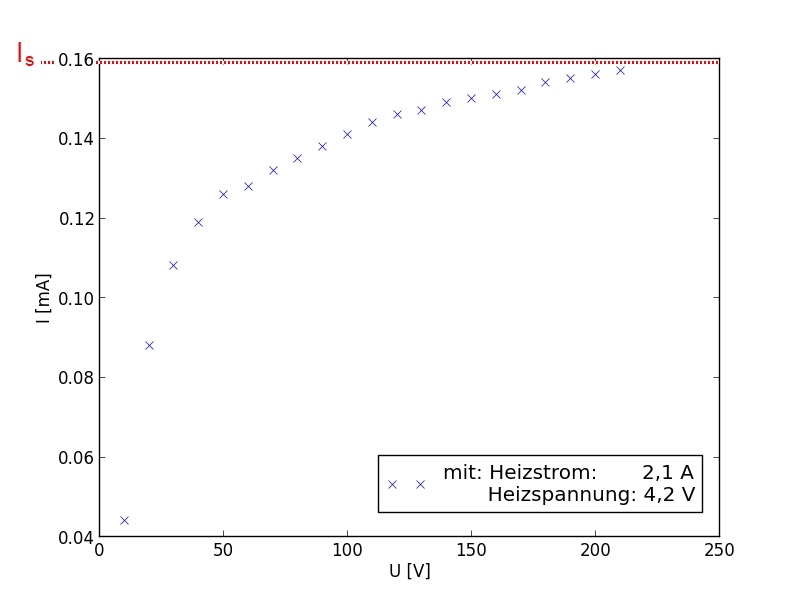
\includegraphics[scale=0.75]{pica1.jpg}
		\caption{Kennlinie 1 (Heizwerte: 4,2V; 2,1A)}
		\label{pica1}
		\end{center}	
	\end{figure} 	\begin{figure}[h]
		\begin{center}
		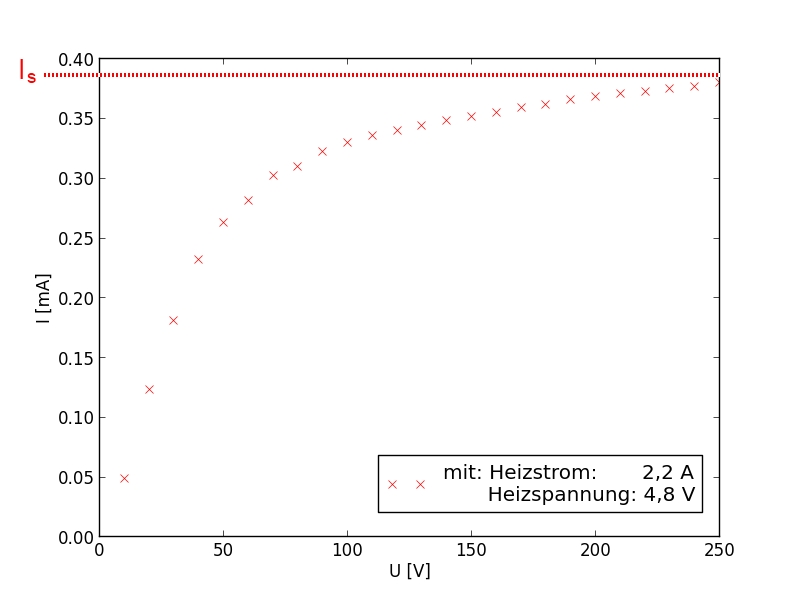
\includegraphics[scale=0.75]{pica2.jpg}
		\caption{Kennlinie 2 (Heizwerte: 4,8V; 2,2A)}
		\label{pica2}
		\end{center}	
	\end{figure} 	\begin{figure}[h]
		\begin{center}
		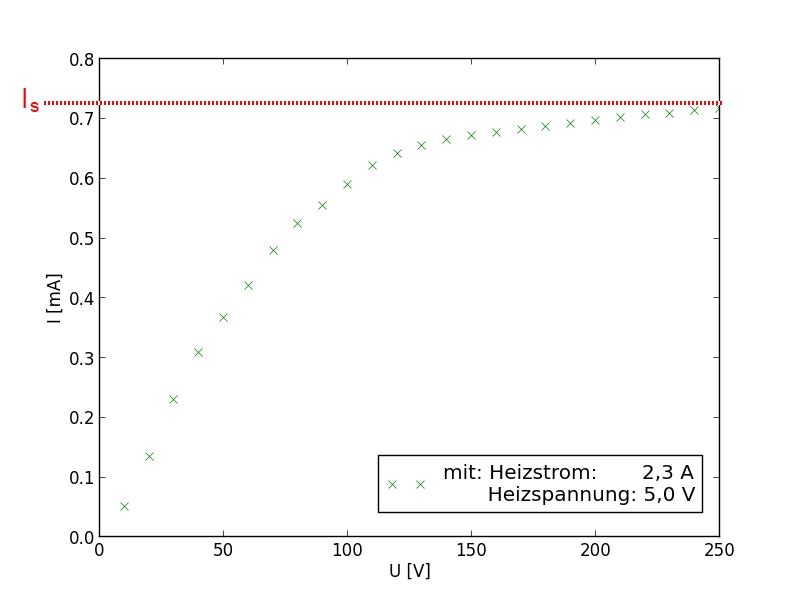
\includegraphics[scale=0.75]{pica3.jpg}
		\caption{Kennlinie 3 (Heizwerte: 5,0V; 2,3A)}
		\label{pica3}
		\end{center}	
	\end{figure} 	\begin{figure}[h]
		\begin{center}
		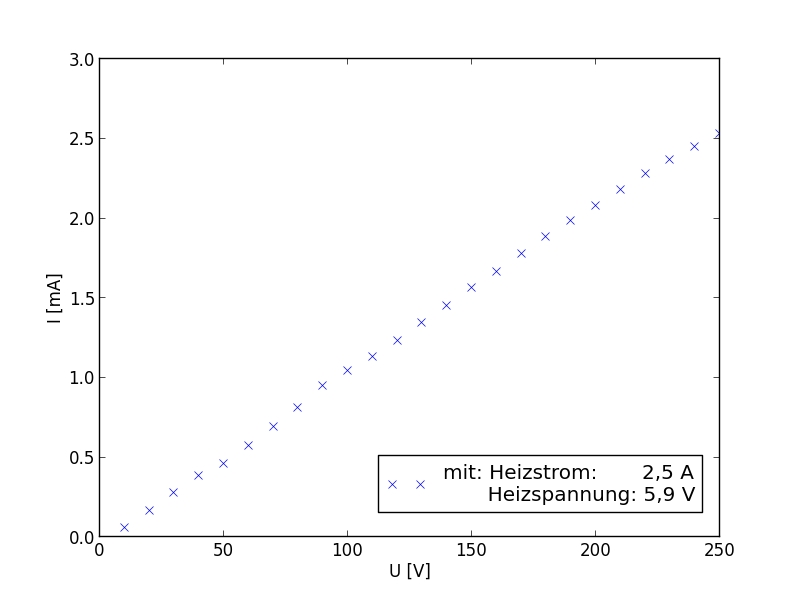
\includegraphics[scale=0.75]{pica4.jpg}
		\caption{Kennlinie 4 (Heizwerte: 5,9V; 2,5A)}
		\label{pica4}
		\end{center}	
	\end{figure} 	\begin{figure}[h]
		\begin{center}
		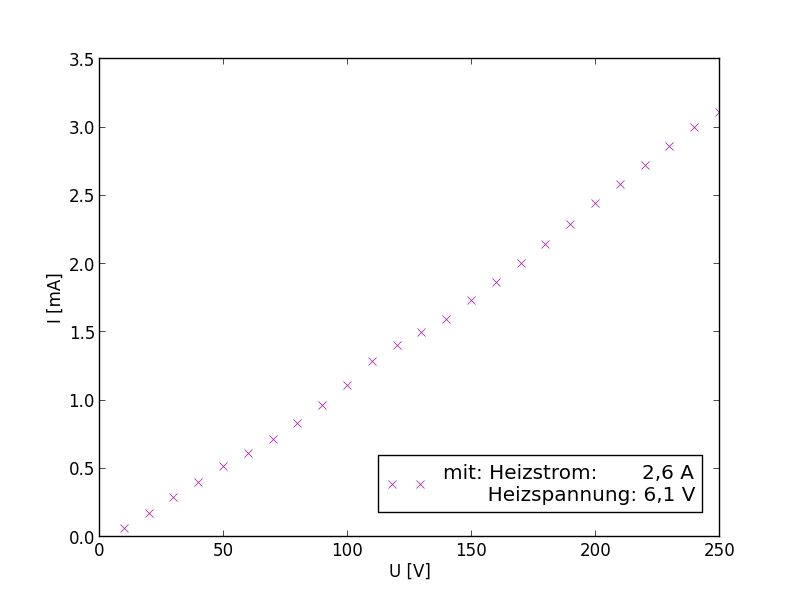
\includegraphics[scale=0.75]{pica5.jpg}
		\caption{Kennlinie 5 (Heizwerte: 6,1V; 2,6A)}
		\label{pica5}
		\end{center}	
	\end{figure} 
Aus den Abbildungen \ref{pica1},\ref{pica2} und \ref{pica3} wurde der Sättingungsstrom 
$I_s$ abgelesen (Tab. \ref{tabis}). Bei den Abbildungen \ref{pica4} und \ref{pica5} war das 
nicht möglich, der Großteil des Sättigungsstromgebietes befand sich außerhalb der 
Messwerte.
\begin{table}[h]
	\begin{center}
		\begin{tabular}{ccc}
			Heizspannung [V] & Heizstrom [A] & Sättigungsstrom [mA]\\ \hline
			4,2 &2,1 &0,16\\
			4,8 &2,2 &0,38\\
			5,0 &2,3 &0,72
		\end{tabular}
		\caption{Sättigungstromwerte}
		\label{tabis}
	\end{center}
\end{table}
\FloatBarrier
\subsection{Langmuir-Schottkysches-Gesetz}
Das Langmuir-Schottkysche Raumladungsgesetz ist solange gültig, bis sich die Kennlinie
dem Sättigungstrom annähert, also das Raumladungsgebiet in das Sättigungsstromgebiet 
übergeht. Für die maximal mögliche Heizleistung passiert das ungefähr bei 200V.
Trägt man die Messwerte logarithmisch auf, so lässt sich der Exponent erkennen (vgl. 
Abb. \ref{picb1}). Der Exponent berechnet sich durch lineare Regression \cite{linreg}
aus Gleichung \ref{eqb1} beziehungsweise Tabelle \ref{tabblinreg} welche auf Tabelle \ref{taba5} aufbaut.
\begin{align}
I&\sim U^\alpha \\
\Leftrightarrow ln(I)&\sim ln(U)*\alpha \label{eqb1}
\end{align}
\begin{table}[h]
	\begin{center}
		\begin{tabular}{cccc}
			U[V] & I[mA] & ln(U) & ln(I)\\ \hline
			10	&0,063& 2,30& -2,765\\                  
			20	&0,170& 2,99& -1,772\\
			30	&0,288& 3,40& -1,245\\
			40	&0,398& 3,68& -0,921\\
			50	&0,514& 3,91& -0,666\\
			60	&0,606& 4,09& -0,501\\
			70	&0,711& 4,24& -0,341\\
			80	&0,829& 4,38& -0,188\\
			90	&0,958& 4,49& -0,043\\
			100	&1,107& 4,60& 0,102\\
			110	&1,282& 4,70& 0,248\\
			120	&1,399& 4,78& 0,336\\
			130	&1,494& 4,86& 0,402\\
			140	&1,593& 4,94& 0,466\\
			150	&1,730& 5,01& 0,548\\
			160	&1,865& 5,07& 0,623\\
			170	&2,000& 5,13& 0,693\\
			180	&2,140& 5,19& 0,761\\
			190	&2,290& 5,24& 0,829\\
		\end{tabular}
		\caption{Logarithmen zur Kennlinie 5 (Heizwerte: 6,1V; 2,6A)}
		\label{tabblinreg}
	\end{center}
\end{table}
\FloatBarrier
Aus der linearen Regression nach \cite{linreg} berechnet sich der gesuchte Exponent $\alpha$ beziehungsweise die Ausgleichskurve (Abb. \ref{picb1}).
\begin{align}
t&=a*x+b \\
a&=\alpha=1,18 \\
b&=-5.3443 \\
\Rightarrow I&=U^\alpha*e^b 
\end{align}
	\begin{figure}[h]
		\begin{center}
		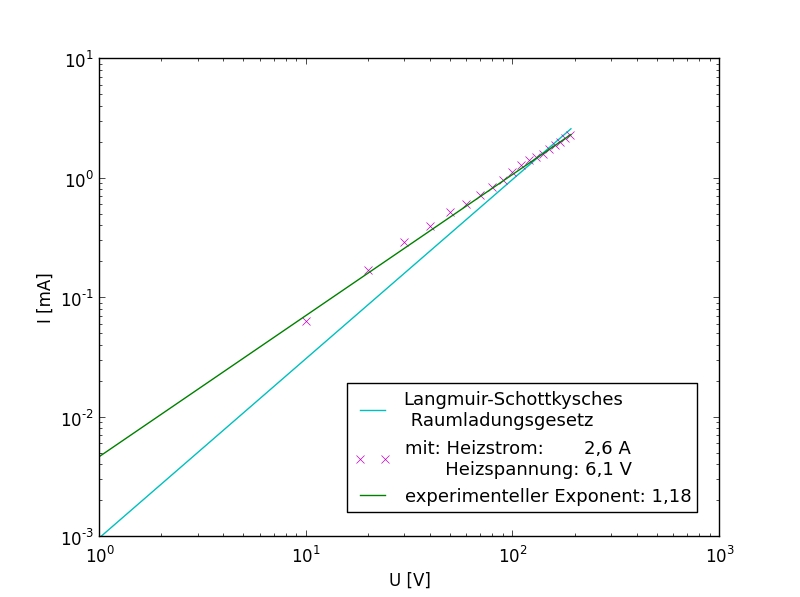
\includegraphics[scale=0.75]{picb1.jpg}
		\caption{Strom-Spannungs-Beziehung}
		\label{picb1}
		\end{center}	
	\end{figure}
\FloatBarrier
\subsection{Kathodentemperatur im Anlaufstromgebiet}

\subsection{Kathodentemperatur bei Saugspannung}

\subsection{Austrittsarbeit des Kathodenmaterials}



